\documentclass{article}

\usepackage{../../common}

\graphicspath{
  {../../../media/images/}
}
\addbibresource{../../references.bib}

\title{Prirodzené čísla a počtové výkony s prirodzenými číslami}
\begin{document}

\maketitle

Čísla $1$, $2$, $3$, $4$\dots\ sa nazývajú \textbf{prirodzené čísla}. Prirodzené čísla sa používajú na počítanie množstva vecí (jeden, dva, tri\dots) a na označenie poradia (prvý, druhý, tretí\dots). Najčastejšie sa označujú symbolom $\mathbb{N}$. V niektorých prípadoch sa uvádza aj číslo $0$ ako prirodzené číslo, vtedy používame na označenie prirodzených čísel symbol $\mathbb{N}_0$.

Prirodzené čísla patria medzi \textbf{základné matematické pojmy}. Na ich poznaní sa stavajú ďalšie matematické poznatky, ako sú celé čísla, zlomky, desatinné čísla atď. Nazývajú sa prirodzené, pretože \textbf{vznikli prirodzenou potrebou ľudí počítať predmety a určovať ich počet}. Už v dávnej minulosti ich ľudia používali na počítanie zvierat, úrody, ľudí alebo dní, ešte skôr, ako vznikli zložitejšie druhy čísel. Preto dostali názov prirodzené čísla. Sú to čísla, ktoré sa objavili prirodzene v každodennom živote.

Prirodzené čísla používame v matematike dvoma rôznymi spôsobmi. Môžeme ich chápať ako kardinálne čísla a ako ordinálne čísla. Kardinalita (číselnosť, početnosť) vyjadruje počet prvkov v súbore. Kardinalita nezávisí od toho, aké prvky v súbore sú, ale iba od ich počtu. Používame základné číslovky ako napríklad jeden, dva, tri, desať, päťnásť, sto, atď. Ordinalita (poradové číslo, usporiadanie) vyjadruje poradie alebo pozíciu prvku v usporiadanom rade. Má zmysel iba v postupnostiach. Používame radové číslovky ako napríklad prvý, druhý, tretí, štvrtý, stí, atď.

\section{Čítanie a zapisovanie prirodzených čísel}

Prirodzené čísla zapisujeme v desiatkovej číselnej sústave pomocou číslic \(0\), \(1\), \(2\), \(3\), \(4\), \(5\), \(6\), \(7\), \(8\) a \(9\). Čísla môžeme zapisovať v skrátenom alebo rozvinutom tvare. Bežne sa čísla zapisujú v skrátenom tvare, pritom dodržujeme zásadu zapisovania číslic do skupiniek po tri od rádu jednotiek. Podľa počtu číslic (cifier) určujeme, o \textbf{koľkociferné prirodzené číslo} ide. Poznáme napríklad prirodzené čísla:
\begin{itemize}
  \item jednociferné: \(0, 1, 2, 3, 4, 5, 6, 7, 8, 9\),
  \item dvojciferné: \(10, 11, 12, \dots, 97, 98, 99\),
  \item trojciferné: \(100, 101, 102, \dots, 997, 998, 999\) atď.
\end{itemize}
Počet cifier prirodzeného čísla je vždy vyjadrený prirodzeným číslom.

Okrem zápisu čísla pomocou cifier môžeme číslo vyjadriť aj slovne. Pravopis čísloviek sa riadi pravidlami slovenského pravopisu. Niektoré pravidlá sú uvedené nižšie.

\begin{displayquote}
  Dovedna (spolu) sa píšu číslovky v základnom tvare, napr. pätnásť, dvadsaťsedem, stojeden, sedemstodvadsať, tisícpäť, sedemtisícdesať. V zložitých prípadoch možno na zvýšenie prehľadnosti oddeľovať tisícky, stovky a desiatky s jednotkami, napr. 7 283 – sedemtisíc dvesto osemdesiattri, 15 348 848 – pätnásť miliónov tristoštyridsaťosemtisíc osemsto štyridsaťosem.

  Poznámka. – Čísla s viac ako tromi číslicami sa členia do skupín po troch čísliciach od poslednej číslice alebo od desatinnej čiarky doľava, alebo od desatinnej čiarky doprava a jednotlivé skupiny sa oddeľujú medzerou, napr. 5 328, 28 565, 139 824, 2 785 632; 37 582,628; 3,141 592 65. Letopočty sa píšu bez medzery, napr. v roku 1848, na začiatku roka 2001.

  V číslovkách od 21 vyššie píšeme oddelene od ostatnej časti jednotky:

  \begin{enumerate}[label=\alph*)]
  \item pri skloňovaní základných čísloviek, napr. stodvadsiati štyria muži, stodvadsiatich štyroch mužov, so stodvadsiatimi štyrmi mužmi;
  \item v radových číslovkách, napr. stodvadsiaty štvrtý účastník, stodvadsiateho štvrtého účastníka, v tisícdeväťstoosemdesiatom piatom roku.
  \end{enumerate}

  Poznámka. – Číslovky označujúce stovky a tisícky sa píšu spolu, napr. dvesto, sedemsto, tritisíc, dvadsaťsedemtisíc, stoosemdesiatdvatisíc. Spolu sa píšu aj radové číslovky zložené z jednotiek, stovák a tisícok, napr. stoprvý, dvetisícdruhý. Číslovky označujúce milióny, miliardy, bilióny sa píšu oddelene, napr. štyri milióny, päť miliónov, tri miliardy, sedem biliónov.\cite{psp2000}
\end{displayquote}

Pri pomenúvaní veľkých čísel používame čísla od \(1\) do \(999\), ktoré určujú násobok základnej jednotky (tisíc, milión, miliarda, bilión\dots). Najčastejšie sa používajú ako predpony alebo násobky veľkých čísel. Napríklad číslo \(238\ 571\ 690\) čítame ako dvestotridsaťosem miliónov päťstosedemdesiatjeden tisíc šestodeväťdesiat. V tabuľke je prehľad písania čísloviek od jedna do sto.

\begin{table}[H]
  \centering
  \renewcommand{\arraystretch}{1.2}
  \begin{tabular}{|cl|cl|cl|cl|}
    \hline
    1 & Jeden & 26 & Dvadsaťšesť & 51 & Päťdesiatjeden & 76 & Sedemdesiatšesť \\
    \hline
    2 & Dva & 27 & Dvadsaťsedem & 52 & Päťdesiatdva & 77 & Sedemdesiatsedem \\
    \hline
    3 & Tri & 28 & Dvadsaťosem & 53 & Päťdesiattri & 78 & Sedemdesiatosem \\
    \hline
    4 & Štyri & 29 & Dvadsaťdeväť & 54 & Päťdesiatštyri & 79 & Sedemdesiatdeväť \\
    \hline
    5 & Päť & 30 & Tridsať & 55 & Päťdesiatpäť & 80 & Osemdesiat \\
    \hline
    6 & Šesť & 31 & Tridsaťjeden & 56 & Päťdesiatšesť & 81 & Osemdesiatjeden \\
    \hline
    7 & Sedem & 32 & Tridsaťdva & 57 & Päťdesiatsedem & 82 & Osemdesiatdva \\
    \hline
    8 & Osem & 33 & Tridsaťtri & 58 & Päťdesiatosem & 83 & Osemdesiattri \\
    \hline
    9 & Deväť & 34 & Tridsaťštyri & 59 & Päťdesiatdeväť & 84 & Osemdesiatštyri \\
    \hline
    10 & Desať & 35 & Tridsaťpäť & 60 & Šesťdesiat & 85 & Osemdesiatpäť \\
    \hline
    11 & Jedenásť & 36 & Tridsaťšesť & 61 & Šesťdesiatjeden & 86 & Osemdesiatšesť \\
    \hline
    12 & Dvanásť & 37 & Tridsaťsedem & 62 & Šesťdesiatdva & 87 & Osemdesiatsedem \\
    \hline
    13 & Trinásť & 38 & Tridsaťosem & 63 & Šesťdesiattri & 88 & Osemdesiatosem \\
    \hline
    14 & Štrnásť & 39 & Tridsaťdeväť & 64 & Šesťdesiatštyri & 89 & Osemdesiatdeväť \\
    \hline
    15 & Pätnásť & 40 & Štyridsať & 65 & Šesťdesiatpäť & 90 & Deväťdesiat \\
    \hline
    16 & Šestnásť & 41 & Štyridsaťjeden & 66 & Šesťdesiatšesť & 91 & Deväťdesiatjeden \\
    \hline
    17 & Sedemnásť & 42 & Štyridsaťdva & 67 & Šesťdesiatsedem & 92 & Deväťdesiatdva \\
    \hline
    18 & Osemnásť & 43 & Štyridsaťtri & 68 & Šesťdesiatosem & 93 & Deväťdesiattri \\
    \hline
    19 & Devätnásť & 44 & Štyridsaťštyri & 69 & Šesťdesiatdeväť & 94 & Deväťdesiatštyri \\
    \hline
    20 & Dvadsať & 45 & Štyridsaťpäť & 70 & Sedemdesiat & 95 & Deväťdesiatpäť \\
    \hline
    21 & Dvadsaťjeden & 46 & Štyridsaťšesť & 71 & Sedemdesiatjeden & 96 & Deväťdesiatšesť \\
    \hline
    22 & Dvadsaťdva & 47 & Štyridsaťsedem & 72 & Sedemdesiatdva & 97 & Deväťdesiatsedem \\
    \hline
    23 & Dvadsaťtri & 48 & Štyridsaťosem & 73 & Sedemdesiattri & 98 & Deväťdesiatosem \\
    \hline
    24 & Dvadsaťštyri & 49 & Štyridsaťdeväť & 74 & Sedemdesiatštyri & 99 & Deväťdesiatdeväť \\
    \hline
    25 & Dvadsaťpäť & 50 & Päťdesiat & 75 & Sedemdesiatpäť & 100 & Sto \\
    \hline
  \end{tabular}
  \caption{Názvy prirodzených čísel do sto.}
\end{table}

V slovenčine používame na pomenovanie veľkých prirodzených čísel dlhú číselnú sústavu. Dlhá číselná sústava je spôsob pomenovania veľkých čísel, ktorý sa používa na Slovensku a vo viacerých európskych krajinách. V tejto sústave sa názvy čísel striedajú na -lión a -liarda. Každý nový -lión je miliónkrát väčší ako predchádzajúci -lión, medzi dvoma -liónmi sa nachádza príslušná -liarda, ktorá je tisíckrát väčšia.

Existuje aj krátka číselná sústava (short scale), ktorá sa používa najmä v USA, vo väčšine anglicky hovoriacich krajín a v modernej medzinárodnej vedeckej komunikácii. V nej každý nový názov končiaci na -illion predstavuje násobenie o tisíc. Najčastejší zdroj nedorozumenia je slovo billion. V angličtine (krátka sústava) znamená \(1\ 000\ 000\ 000\), teda po slovensky miliarda, nie bilión. V súčasnosti používa Slovensko, Česko, Nemecko, Francúzsko a väčšina kontinentálnej Európy dlhú sústavu, zatiaľ čo USA, Kanada, Austrália a Spojené kráľovstvo používajú krátku sústavu. Pri preklade ekonomických alebo vedeckých textov z angličtiny je preto potrebné venovať týmto názvom zvýšenú pozornosť. V tabuľke je prehľad niektorých názvov veľkých prirodzených čísel.\footnote{Zápis \(10^n\), kde \(n\) je prirodzené číslo, znamená násobenie čísla \(10\) samého sebou \(n\)-krát. Výsledné číslo je jednotka nasledovaná \(n\) nulami.}

\begin{table}[H]
  \centering
  \renewcommand{\arraystretch}{1.2}
  \begin{tabular}{|r|c|l|r|c|l|}
    \hline
    \textbf{Názov} & \textbf{Núl} & \textbf{Číslo} &
    \textbf{Názov} & \textbf{Núl} & \textbf{Číslo} \\
    \hline
    Jedna & 0 & \(1\) &
    Trilión & 18 & \(10^{18}\) \\
    \hline
    Desať & 1 & \(10\) &
    Triliarda & 21 & \(10^{21}\) \\
    \hline
    Sto & 2 & \(100\) &
    Kvadrilión & 24 & \(10^{24}\) \\
    \hline
    Tisíc & 3 & \(1\ 000\) &
    Kvadriliarda & 27 & \(10^{27}\) \\
    \hline
    Desaťtisíc & 4 & \(10\ 000\) &
    Kvintilión & 30 & \(10^{30}\) \\
    \hline
    Stotisíc & 5 & \(100\ 000\) &
    Kvintiliarda & 33 & \(10^{33}\) \\
    \hline
    Milión & 6 & \(1\ 000\ 000\) &
    Sextilión & 36 & \(10^{36}\) \\
    \hline
    Desať miliónov & 7 & \(10\ 000\ 000\) &
    Sextiliarda & 39 & \(10^{39}\) \\
    \hline
    Sto miliónov & 8 & \(100\ 000\ 000\) &
    Septilión & 42 & \(10^{42}\) \\
    \hline
    Miliarda & 9 & \(1\ 000\ 000\ 000\) &
    Septiliarda & 45 & \(10^{45}\) \\
    \hline
    Desať miliárd & 10 & \(10\ 000\ 000\ 000\) &
    Oktilión & 48 & \(10^{48}\) \\
    \hline
    Sto miliárd & 11 & \(100\ 000\ 000\ 000\) &
    Oktiliarda & 51 & \(10^{51}\) \\
    \hline
    Bilión & 12 & \(1\ 000\ 000\ 000\ 000\) &
    Nonilión & 54 & \(10^{54}\) \\
    \hline
    Desať biliónov & 13 & \(10\ 000\ 000\ 000\ 000\) &
    Noniliarda & 57 & \(10^{57}\) \\
    \hline
    Sto biliónov & 14 & \(100\ 000\ 000\ 000\ 000\) &
    Decilión & 60 & \(10^{60}\) \\
    \hline
    Biliarda & 15 & \(1\ 000\ 000\ 000\ 000\ 000\) &
    Deciliarda & 63 & \(10^{63}\) \\
    \hline
    Desať biliárd & 16 & \(10\ 000\ 000\ 000\ 000\ 000\) &
    Google & 100 & \(10^{100}\) \\
    \hline
    Sto biliárd & 17 & \(100\ 000\ 000\ 000\ 000\ 000\) &
    Centilión & 600 & \(10^{600}\) \\
    \hline
  \end{tabular}
  \caption{Názvy veľkých prirodzených čísel.}
\end{table}

Príklady zápisu a čítania niektorých prirodzených čísel:
\begin{itemize}
  \item \(42\), čítame: štyridsaťdva
  \item \(125\), čítame: stodvadsaťpäť
  \item \(3\ 850\), čítame: tritisíc osemstopäťdesiat
  \item \(56\ 823\), čítame: päťdesiatšesťtisíc osemstodvadsaťtri
  \item \(804\ 256\), čítame: osemstoštyritisíc dvestopäťdesiatšesť
  \item \(1\ 354\ 672\), čítame: jeden milión tristopäťdesiatštyritisíc šesťstosedemdesiatdva
  \item \(4\ 506\ 321\), čítame: štyri milióny päťstotisíc šesťtisíc tristo dvadsaťjeden
  \item \(12\ 450\ 678\), čítame: dvanásť miliónov štyristopäťdesiattisíc šesťstosedemdesiatosem
  \item \(35\ 627\ 002\), čítame: tridsaťpäť miliónov šesťstodvadsaťsedemtisíc dva
  \item \(78\ 305\ 412\), čítame: sedemdesiatosem miliónov tristopäťtisíc štyristodvanásť
  \item \(125\ 678\ 904\), čítame: stodvadsaťpäť miliónov šesťstosedemdesiatosemtisíc deväťstoštyri
  \item \(832\ 102\ 098\), čítame: osemstotridsaťdva miliónov stodvatisíc deväťdesiatosem
  \item \(1\ 250\ 000\ 000\), čítame: jedna miliarda dvestopäťdesiat miliónov
  \item \(3\ 456\ 789\ 012\), čítame: tri miliardy štyristopäťdesiatšesť miliónov sedemstoosemdesiatdeväťtisíc dvanásť
  \item \(25\ 804\ 321\ 765\), čítame: dvadsaťpäť miliárd osemstoštyri miliónov tristodvadsaťjedentisíc sedemstošesťdesiatpäť
  \item \(100\ 000\ 000\ 000\), čítame: sto miliárd
  \item \(7\ 250\ 600\ 400\ 000\), čítame: sedem biliónov dvestopäťdesiat miliárd šesťsto miliónov štyristotisíc
  \item \(45\ 678\ 901\ 234\ 567\), čítame: štyridsaťpäť biliónov šesťstoosemdesiatsedem miliárd deväťsto jeden miliónov dvestotridsaťštyritisíc päťstošesťdesiatsedem
\end{itemize}

\section{Zobrazenie prirodzených čísel na číselnej osi}

\textbf{Číselná os} je priamka, na ktorej zobrazujeme čísla. Sú na nej usporiadané čísla podľa ich veľkosti. Používa sa na znázornenie čísel a na jednoduchšie porovnávanie, ktoré číslo je väčšie alebo menšie. Obrazom čísla je bod na číselnej osi. Obrazmi prirodzených čísel sú body ležiace na číselnej osi vpravo od bodu nula. Bod, ktorý patrí menšiemu číslu, leží bližšie k nule.

Znázornenie čísel na číselnej osi si môžeme prispôsobiť podľa toho, ktoré čísla potrebujeme zobraziť. Pri znázornení musia byť splnené nasledovné podmienky:
\begin{itemize}
  \item Každému číslu zodpovedá práve jeden bod na číselnej osi a každému bodu na osi zodpovedá práve jedno číslo.
  \item Vzdialenosť medzi dvoma susednými číslami musí byť vždy rovnaká.
  \item Smerom doprava sa čísla zväčšujú a smerom doľava zmenšujú.
\end{itemize}
Priamka môže byť na konci označená šípkou, ktorá naznačuje, že pokračuje do nekonečna.

Príklady niektorých znázornení prirodzených čísel na číselnej osi:

\begin{center}
  Počítame od nuly po jednotkách. \vspace{5mm}

  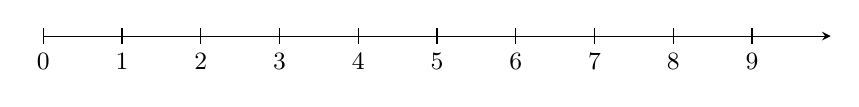
\begin{tikzpicture}[>=stealth]
    \draw[->] (0,0) -- (10,0);
    \foreach \x in {0,1,...,9}
    {
      \draw (\x,0.1) -- (\x,-0.1);
      \node[below] at (\x,-0.1) {\small $\x$};
    }
  \end{tikzpicture}
\end{center}

\begin{center}
  Počítame od nuly po desiatkach. \vspace{5mm}

  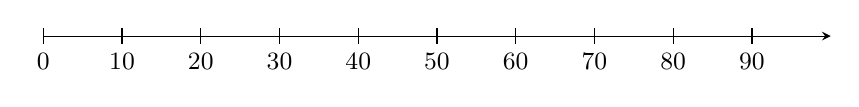
\begin{tikzpicture}[>=stealth]
    \draw[->] (0,0) -- (10,0);
    \foreach \x/\label in {0/0,1/10,2/20,3/30,4/40,5/50,6/60,7/70,8/80,9/90}
    {
      \draw (\x,0.1) -- (\x,-0.1);
      \node[below] at (\x,-0.1) {\small \label};
    }
  \end{tikzpicture}
\end{center}

\begin{center}
  Počítame od nuly po stovkách. \vspace{5mm}

  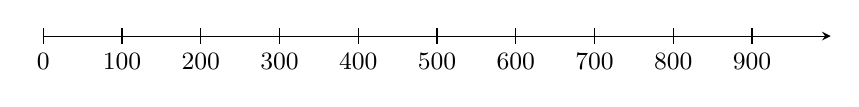
\begin{tikzpicture}[>=stealth]
    \draw[->] (0,0) -- (10,0);
    \foreach \x/\label in {0/0,1/100,2/200,3/300,4/400,5/500,6/600,7/700,8/800,9/900}
    {
      \draw (\x,0.1) -- (\x,-0.1);
      \node[below] at (\x,-0.1) {\small \label};
    }
  \end{tikzpicture}
\end{center}

\begin{center}
  Počítame od nuly po dvojkách. \vspace{5mm}

  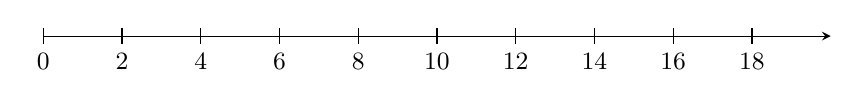
\begin{tikzpicture}[>=stealth]
    \draw[->] (0,0) -- (10,0);
    \foreach \x/\label in {0/0,1/2,2/4,3/6,4/8,5/10,6/12,7/14,8/16,9/18}
    {
      \draw (\x,0.1) -- (\x,-0.1);
      \node[below] at (\x,-0.1) {\small \label};
    }
  \end{tikzpicture}
\end{center}

\begin{center}
  Počítame od nuly po sedmičkách. \vspace{5mm}

  \begin{tikzpicture}[>=stealth]
    \draw[->] (0,0) -- (10,0);
    \foreach \x/\label in {0/0,2/7,4/14,6/21,8/35}
      {
        \draw (\x,0.1) -- (\x,-0.1);
        \node[below] at (\x,-0.1) {\small \label};
      }
  \end{tikzpicture}
\end{center}

\begin{center}
  Počítame od čísla 45 po päťkách. \vspace{5mm}

  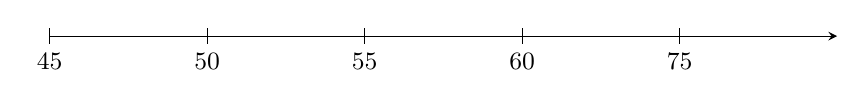
\begin{tikzpicture}[>=stealth]
    \draw[->] (0,0) -- (10,0);
    \foreach \x/\label in {0/45,2/50,4/55,6/60,8/75}
      {
        \draw (\x,0.1) -- (\x,-0.1);
        \node[below] at (\x,-0.1) {\small \label};
      }
  \end{tikzpicture}
\end{center}

\begin{center}
  Počítame od čísla 10 po desiatkách. Znázorňujeme každé druhé číslo. \vspace{5mm}

  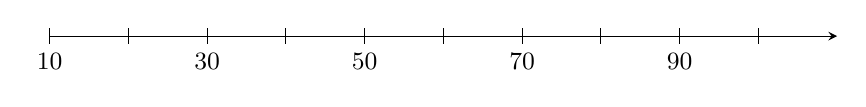
\begin{tikzpicture}[>=stealth]
    \draw[->] (0,0) -- (10,0);
    \foreach \x/\label in {0/10,1/,2/30,3/,4/50,5/,6/70,7/,8/90,9/}
      {
        \draw (\x,0.1) -- (\x,-0.1);
        \node[below] at (\x,-0.1) {\small \label};
      }
  \end{tikzpicture}
\end{center}

\begin{center}
  Počítame od čísla 2 po šestkách. Znázorňujeme každé tretie číslo. \vspace{5mm}

  \begin{tikzpicture}[>=stealth]
    \draw[->] (0,0) -- (10,0);
    \foreach \x/\label in {0/2,1/,2/,3/20,4/,5/,6/38,7/,8/,9/56}
      {
        \draw (\x,0.1) -- (\x,-0.1);
        \node[below] at (\x,-0.1) {\small \label};
      }
  \end{tikzpicture}
\end{center}

\begin{center}
  Počítame od čísla 90 po deviatkách. Znázorňujeme každé tretie číslo od čísla 108. \vspace{5mm}

  \begin{tikzpicture}[>=stealth]
    \draw[->] (0,0) -- (10,0);
    \foreach \x/\label in {0/,1/,2/108,3/,4/,5/135,6/,7/,8/162,9/}
      {
        \draw (\x,0.1) -- (\x,-0.1);
        \node[below] at (\x,-0.1) {\small \label};
      }
  \end{tikzpicture}
\end{center}


\section{Porovnávanie a usporiadanie prirodzených čísel}

Porovnávanie prirodzených čísel znamená určiť, ktoré číslo je väčšie, menšie alebo či sú obe čísla rovnaké. V desiatkovej číselnej sústave je desať rôznych číslic v poradí od najmenšej po najväčšiu: \(0\), \(1\), \(2\), \(3\), \(4\), \(5\), \(6\), \(7\), \(8\) a \(9\). Každá číslica vyjadruje určitú hodnotu. Väčšie čísla sú tvorené kombináciou týchto desiatich číslic.

Každé číslo dokážeme usporiadať tak, aby výsledná postupnosť čísel bola zoradená podľa veľkosti. Usporiadanie znamená vytvorenie určitej postupnosti. Usporiadaním prirodzených čísel vytvoríme postupnosť čísel \(0\), \(1\), \(2\), \(3\), \(4\), \(5\), \(6\), \(7\), \(8\), \(9\), \(10\), \(11\), \(12\)\dots atď. Susedné čísla sa líšia o hodnotu jeden. Graficky by sa táto postupnosť dala znázorniť ako číselná os.

\begin{center}
  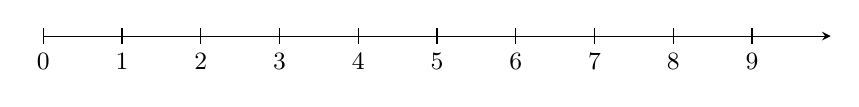
\begin{tikzpicture}[>=stealth]
    \draw[->] (0,0) -- (10,0);
    \foreach \x in {0,1,...,9}
    {
      \draw (\x,0.1) -- (\x,-0.1);
      \node[below] at (\x,-0.1) {\small $\x$};
    }
  \end{tikzpicture}
\end{center}

Usporiadania môžu byť dvojakého typu: od najmenšieho čísla po najväčšie číslo, nazývané ako vzostupné, a od najväčšieho čísla po najmenšie číslo, nazývané ako zostupné. Pre potreby porovnávania sa používa vzostupné usporiadanie čísel.

Vzostupné usporiadanie prirodzených čísel umožňuje zaviesť vzťahy, pomocou ktorých porovnávame čísla na základe ich veľkosti. Pre dve prirodzené čísla \(a\) a \(b\) môžeme zaviesť nasledovné vzťahy:
\begin{itemize}
  \item Číslo \(a\) je väčšie ako číslo \(b\), ak sa na číselnej osi nachádza napravo od čísla \(b\).
  \item Číslo \(a\) je menšie ako číslo \(b\), ak sa na číselnej osi nachádza naľavo od čísla \(b\).
  \item Číslo \(a\) sa rovná číslu \(b\), ak sa na číselnej osi nachádzajú v tom istom bode.
\end{itemize}
Zhrnutím do jednej vety môžeme povedať, že z dvoch prirodzených čísel je väčšie to, ktorého obraz na číselnej osi je ďalej od nuly. Na základe tohto môžeme definovať šesť typov porovnávania čísel: väčší ako, menší ako, rovná sa, väčší alebo rovná sa, menší alebo rovná sa a nerovná sa. V tabuľke sú ku každému porovnávaniu priradené aj symbolické zápisy.

\begin{table}[H]
  \centering
  \renewcommand{\arraystretch}{1.3}
  \begin{tabular}{|l|c|}
    \hline
    \multicolumn{1}{|c|}{Porovnávanie} &
    \multicolumn{1}{c|}{Znak} \\
    \hline
    Väčší ako & \(>\) \\
    Menší ako & \(<\) \\
    Rovná sa & \(=\) \\
    Väčší alebo rovná sa & \(\geq\) \\
    Menší alebo rovná sa & \(\leq\) \\
    Nerovná sa & \(\neq\) \\
    \hline
  \end{tabular}
  \caption{Prehľad porovnávaní a ich symbolický zápis.}
\end{table}

Pre dve prirodzené čísla \(a\) a \(b\), kde:
\begin{itemize}
  \item číslo \(a\) je väčšie ako číslo \(b\), platí \(a > b\),
  \item číslo \(a\) je menšie ako číslo \(b\), platí \(a < b\),
  \item číslo \(a\) sa rovná číslu \(b\), platí \(a = b\),
  \item číslo \(a\) je väčšie alebo sa rovná číslu \(b\), platí \(a \geq b\),
  \item číslo \(a\) je menšie alebo sa rovná číslu \(b\), platí \(a \leq b\),
  \item číslo \(a\) sa nerovná číslu \(b\), platí \(a \neq b\).
\end{itemize}
Porovnávať dve ľubovoľné prirodzené čísla môžeme týmto postupom v tomto poradí:
\begin{enumerate}[label=\arabic*)]
  \item Číslo s väčším počtom číslic je väčšie.
  \item Ak majú čísla rovnaký počet číslic, porovnávame ich číslice zľava doprava. Číslo je väčšie, ak má väčšiu číslicu v prvej nezhode.
  \item Ak sú všetky číslice rovnaké, čísla sú rovnaké.
\end{enumerate}

\section{Zaokrúhľovanie prirodzených čísel}

Zaokrúhľovanie je postup, kde nahrádzame číslo iným menej presným číslom, ktoré je jednoduchšie na čítanie, zapisovanie alebo počítanie. Používa sa vtedy, keď nepotrebujeme pracovať s úplne presnou hodnotu. Zaokrúhľovanie používame pri bežných odhadoch (napríklad koľko približne stojí nákup), pri meraní (dĺžka, hmotnosť, teplota), v štatistikách alebo pri rýchlych výpočtoch. Pri zaokrúhľovaní sa snažíme zmeniť číslo čo najmenej, aby sa výsledok čo najpresnejšie približoval k reálnej hodnote.

Pri zaokrúhľovaní nahradíme zaokrúhľované číslo jemu blízkym číslom. Zaokrúhľujeme najčastejšie na určitý číselný rád. Zaokrúhľovaním na určitý čiselný rád musíme dostať číslo, ktoré je násobkom tohto číselného rádu. Pri zaokrúhľovaní čísla na desiatky bude výsledok násobkom desiatky, pri zaokrúhľovaní čísla na stovky bude výsledok násobkom stovky atď. Na aký násobok číselného rádu zaokrúhľujeme číslo má vplyv číslica nižšieho rádu, ktorá sa nazýva rozhodujúca číslica. Pri zaokrúhľovaní na desiatky je rozhodujúca číslica rádu jednotiek, pri zaokrúhľovaní na stovky je rozhodujúca číslica rádu desiatok atď. Výsledkom zaokrúhľovania je číslo, v ktorom sú rozhodujúca číslica a všetky číslice nižších rádov nahradené nulami.

Podľa toho, či zaokrúhľujeme na menší alebo väčší násobok, rozlišujeme tri typy zaokrúhľovania čísel: zaokrúhľovanie nadol, zaokrúhľovanie nahor a aritmetické zaokrúhľovanie.
\begin{itemize}
  \item Pri zaokrúhľovaní nadol je výsledkom najbližšie prirodzené číslo, ktoré je menšie alebo sa rovná zaokrúhľovanému číslu.
  \item Pri zaokrúhľovaní nahor je výsledkom najbližšie prirodzené číslo, ktoré je väčšie alebo sa rovná zaokrúhľovanému číslu.
  \item Pri aritmetickom zaokrúhľovaní sa zaokrúhľuje buď nahor alebo nadol. Ak rozhodujúca číslica je \(0\), \(1\), \(2\), \(3\), \(4\), zaokrúhľujeme nadol. Ak rozhodujúca číslica je \(5\), \(6\), \(7\), \(8\), \(9\), zaokrúhľujeme nahor. Prívlastok aritmetické sa zvykne vynechávať, teda ak je uvedené "zaokrúhlite", ide o aritmetické zaokrúhľovanie.
\end{itemize}
Aritmetické zaokrúhľovanie je bežný spôsob zaokrúhľovania. Poskytuje najbližší násobok desiatky, stovky, tisícky atď. k pôvodnému číslu. Má ale jeden problém pri číslach, ktoré sú rovnakej vzdialenosti na číselnej osi od najbližších násobkoch. Nastáva to pri číslach \(5\) pri zaokrúhľovaní na desiatky, \(50\) pri zaokrúhľovaní na stovky, \(500\) pri zaokrúhľovaní na tisícky atď. V týchto prípadoch platí zásada, že zaokrúhľujeme nahor.

Zaokrúhľovanie ako matematickú operáciu zapisujeme pomocou znaku \enquote{\(\, \doteq \,\)}. Pôvodné číslo, ktoré zaokrúhľujeme, sa píše na ľavej strane znaku a číslo, ktoré je výsledkom zaokrúhľovania, sa píše na pravej strane. Napríklad číslo \(45\) zaokrúhlené na desiatky sa zapíše ako \(45 \doteq 50\). To, na aký číselný rád zaokrúhľujeme, sa v zápise nešpecifikuje, táto informácia musí vychádzať z kontextu, v ktorom sa zápis nachádza.

K 1. júlu 2022 nadobudla účinnosť novela zákona o cenách, ktorá má za cieľ obmedziť obeh jednocentových a dvojcentových mincí na Slovensku. Tieto mince ale naďalej zostali zákonným platidlom a je ich tak možné vydávať aj prijímať. Pri platbe nákupu v hotovosti sa uplatňuje zaokrúhľovanie eurocentov. Keď je konečná suma v obchode necelým násobkom 5 centov, zaokrúhli sa podľa poslednej číslice tak, ako je uvedené v tabuľke.

\begin{table}[H]
  \centering
  \renewcommand{\arraystretch}{1.3}
  \begin{tabular}{|c|c|c|}
    \hline
    Posledná číslica & Zaokrúhľovanie & Príklad \\
    \hline
    1 alebo 2 & Nadol na 0 & \euro 1.22 \(\rightarrow\) \euro 1.20 \\
    3 alebo 4 & Nahor na 5 & \euro 1.24 \(\rightarrow\) \euro 1.25 \\
    6 alebo 7 & Nadol na 5 & \euro 1.37 \(\rightarrow\) \euro 1.35 \\
    8 alebo 9 & Nahor na 10 & \euro 1.89 \(\rightarrow\) \euro 1.90 \\
    \hline
  \end{tabular}
  \caption{Tabuľka zaokrúhľovania eurocentov.}
\end{table}

\section{Operácie s prirodzenými číslami}

Operácia je postup, podľa ktorého z jedného alebo viacerých matematických výrazov (napríklad čísel) vytvoríme nový matematický objekt. Každá operácia má svoj vstup a výstup. Vstupom pre operácie sú jeden, dva alebo viac výrazov, ktoré nazývame operandy. Výstupom operácie je výsledok, ktorý dostaneme po vykonaní tejto operácie. Operáciu označujeme zástupným znakom, ktorý nazývame operátor.

Poznáme štyri základné aritmetické operácie s prirodzenými číslami: sčítanie, odčítanie, násobenie, delenie.

\begin{table}[H]
  \centering
  \renewcommand{\arraystretch}{1.3}
  \begin{tabular}{c|c|c|c|c}
    Operácia & Operand & Operátor & Operand & Výsledok \\
    \hline
    Sčítanie & Sčítanec & \(+\) & Sčítanec & Súčet \\
    Odčítanie & Menšenec & \(-\) & Menšiteľ & Rozdiel \\
    Násobenie & Činiteľ & \(\cdot\) & Činiteľ & Súčin \\
    Delenie & Delenec & \(:\) & Deliteľ & Podiel \\
  \end{tabular}
  \caption{Tabuľka štyroch základných aritmetických operácií s prirodzenými číslami.}
\end{table}

Tieto aritmetické operácie priraďujú dvom operandom jeden výsledok. Vo výrazoch s viacnásobnými operáciami ako napríklad \(4 + 5 + 11 + 7\) sa počíta postupne zľava doprava, sčítajú sa prvé dve čísla, výsledok sa sčíta s tretím číslom, tento výsledok sa sčíta so štvrtým číslom atď. Nie je možné spočítať naraz tri a viac čísel.

V matematike sa všetky tieto aritmetické operácie nad prirodzenými číslami dajú presne definovať pomocou dvoch pojmov: nasledovník a predchodca. Nasledovník prirodzeného čísla je číslo, ktoré nasleduje za toto prirodzené číslo v postupnosti čísel \(0\), \(1\), \(2\), \(3\), \(4\), \(5\), \(6\), \(7\), \(8\), \(9\), \(10\), \(11\), \(12\)\dots Každé prirodzené číslo má svojho nasledovníka. Prirodzené číslo \(0\) má nasledovníka číslo \(1\), prirodzené číslo \(1\) má nasledovníka číslo \(2\) atď. S pojmom nasledovníka súvisí aj pojem predchodca. Predchodca prirodzeného čísla je číslo, ktorého nasledovník je pôvodné prirodzené číslo. Napríklad predchodca čísla \(2\) je číslo \(1\), predchodca čísla \(1\) je číslo \(0\). Číslo \(0\) nemá predchodcu (v prirodzených číslach).

\subsection{Sčítanie prirodzených čísel}

Sčítanie je operácia, pri ktorej spájame dve alebo viac množstiev do jedného celku. Čísla, ktoré sčítavame, sa nazývajú sčítance a výsledok sčítania sa nazýva súčet. Slovom súčet označujeme tiež zápis sčítania. Operátor sčítania je znak plus \enquote{\(\, + \,\)}. Sčítanie čísla \(a\) a čísla \(b\) zapisujeme ako \(a + b\).

Sčítanie prirodzených čísel môžeme definovať pomocou dvoch základných pravidiel:
\[
\begin{aligned}
  \text{(1)}\quad a + 0 &= a, \\
  \text{(2)}\quad a + 1 &= \text{nasledovník}(a).
\end{aligned}
\]
Pravidlo (1) hovorí, že ak k ľubovoľnému prirodzenému číslu \(a\) pripočítame nulu, hodnota čísla sa nezmení. Nula teda pri sčítaní neovplyvňuje výsledok. Pravidlo (2) vyjadruje vzťah medzi sčítaním a pojmom nasledovníka. Ak k číslu \(a\) pripočítame jednotku, dostaneme jeho nasledovníka. Zároveň platí aj opak, akékoľvek prirodzené číslo väčšie ako nula môžeme vyjadriť ako súčet predchodcu a jednotky. Napríklad číslo \(5\) môžeme vyjadriť ako \(4 + 1\). Takto môžeme každé prirodzené číslo vyjadriť ako súčet jednotiek, kde počet jednotiek dáva výsledné číslo. Prevod čísla \(5\) na jednotky vypadá nasledovne:
\[
\begin{aligned}
  &5, \\
  &4 + 1, \\
  &3 + 1 + 1, \\
  &2 + 1 + 1 + 1, \\
  &1 + 1 + 1 + 1 + 1. \\
\end{aligned}
\]
Tieto dve pravidlá nám umožňujú definovať súčet ľubovoľných dvoch prirodzených čísel. Ak chceme vypočítať súčet čísel \(a\) a \(b\), môžeme číslo \(b\) chápať ako opakované pridávanie jednotky. Každá pripočítaná jednotka posunie číslo \(a\) k jeho ďalšiemu nasledovníkovi. Ako konkrétny príklad si môžeme zobrať čísla \(2\) a \(5\).
\[
\begin{aligned}
  &2 + 5, \\
  &2 + 4 + 1, \\
  &2 + 3 + 1 + 1, \\
  &2 + 2 + 1 + 1 + 1, \\
  &2 + 1 + 1 + 1 + 1 + 1, \\
  &3 + 1 + 1 + 1 + 1, \\
  &4 + 1 + 1 + 1, \\
  &5 + 1 + 1, \\
  &6 + 1, \\
  &7.
\end{aligned}
\]
Výsledok sčítania \(2 + 5\) je číslo \(7\). Sčítanie teda môžeme chápať ako postupné vytváranie nasledovníkov: druhé číslo \(b\) určuje, koľkokrát máme od čísla \(a\) prejsť k jeho nasledovníkom. Výsledok sčítania dvoch prirodzených čísel \(a + b\) je číslo \(c\), ktoré dostaneme po prevedení čísla \(b\) na súčet jednotiek a postupným prevodom čísla \(a\) na nasledovníkov. Pri viacciferných číslach je táto metóda transformácie čísla na jednotky a následného vytvárania nasledovníkov veľmi nepraktická a zdĺhavá, preto existujú efektívne algoritmy na sčítanie ľubovoľných prirodzených čísel.

Pri zámene sčítancov v sčítaní môžeme túto postupnosť jednotiek porovnať medzi sebou. Ak je výsledok tá istá postupnosť sčítania jednotiek, súčty dvoch čísel sa musia rovnať. Napríklad zámenou sčítancov v sčítaní \(2 + 3\) dostaneme \(3 + 2\). Po prevode oboch operácií dostaneme:
\[
\begin{aligned}
  &2 + 3, \\
  &2 + 2 + 1, \\
  &2 + 1 + 1 + 1, \\
  &1 + 1 + 1 + 1 + 1. \\
\end{aligned}
\hspace{5em}
\begin{aligned}
  &3 + 2, \\
  &3 + 1 + 1, \\
  &2 + 1 + 1 + 1, \\
  &1 + 1 + 1 + 1 + 1. \\
\end{aligned}
\]
Oba prevody vedú na tú istú postupnosť sčítania jednotiek, ich súčty sa teda musia rovnať. Táto vlasnosť sa nazýva komutatívnosť a je to jedna zo základných vlastností operácie sčítania.

Pri sčítaní jednociferných čísel je časovo najvýhodnejšie zapamätať si základné spoje ščítania, ktoré sú ukázané v tabuľke. Pri súčtoch niektorých cifier si môžeme všimnúť, že potrebujeme v ráde desiatok zapísať jednotku. Túto jednotku budeme musieť pri sčítaní dvoch väčších čísel zarátavať do výsledku.
\begin{table}[H]
  \centering
  \renewcommand{\arraystretch}{1.3}
  \newcolumntype{C}{>{\centering\arraybackslash}m{1em}}
  \begin{tabular}{C|CCCCCCCCCC}
    \(+\) & 0 & 1 & 2 & 3 & 4 & 5 & 6 & 7 & 8 & 9 \\
    \hline
    0 & 0 & 1 & 2 & 3 & 4 & 5 & 6 & 7 & 8 & 9 \\
    1 & 1 & 2 & 3 & 4 & 5 & 6 & 7 & 8 & 9 & 10 \\
    2 & 2 & 3 & 4 & 5 & 6 & 7 & 8 & 9 & 10 & 11 \\
    3 & 3 & 4 & 5 & 6 & 7 & 8 & 9 & 10 & 11 & 12 \\
    4 & 4 & 5 & 6 & 7 & 8 & 9 & 10 & 11 & 12 & 13 \\
    5 & 5 & 6 & 7 & 8 & 9 & 10 & 11 & 12 & 13 & 14 \\
    6 & 6 & 7 & 8 & 9 & 10 & 11 & 12 & 13 & 14 & 15 \\
    7 & 7 & 8 & 9 & 10 & 11 & 12 & 13 & 14 & 15 & 16 \\
    8 & 8 & 9 & 10 & 11 & 12 & 13 & 14 & 15 & 16 & 17 \\
    9 & 9 & 10 & 11 & 12 & 13 & 14 & 15 & 16 & 17 & 18 \\
  \end{tabular}
  \caption{Tabuľka súčtov čísel od \(0\) do \(9\).}
\end{table}

Na sčítanie ľubovoľných viacciferných prirodzených čísel používame nasledujúci algoritmus:
\begin{enumerate}[label=\arabic*)]
  \item Začneme od číslic najnižšieho rádu (jednotiek).
  \item Opakujeme cyklus, kým nespracujeme všetky rády oboch sčítancov:
  \begin{enumerate}
    \item Sčítame číslice oboch sčítancov v aktuálnom ráde, vzniknutý súčet bude medzivýsledok. Ak existuje prenos z predchádzajúceho cyklu, pripočítame ho k tomuto medzivýsledku.
    \item Číslicu na mieste jednotiek medzivýsledku zapíšeme do príslušného rádu výsledku sčítania.
    \item Ak je medzivýsledok väčší alebo rovný \(10\), prenesieme číslicu rádu desiatok do nasledujúceho vyššieho rádu.
    \item Pokračujeme spracovaním nasledujúceho vyššieho rádu.
  \end{enumerate}
  \item Výsledok je súčet oboch sčítancov.
\end{enumerate}
Pre ľahšiu manipuláciu číslic a ich rádov sa pri tomto algoritme využíva písomné sčítanie.

\subsubsection{Písomné sčítanie prirodzených čísel} 

Písomné sčítanie čísel je spôsob sčítania, pri ktorom zapisujeme čísla pod seba podľa rádov (jednotky pod jednotkami, desiatky pod desiatkami, stovky pod stovkami atď.) a sčítavame ich postupne sprava doľava.

Dva sčítance sa zapíšu jeden pod druhým tak, aby každý rád sčítancov bol v tom istom stĺpci. Pod druhý sčítanec sa urobí vodorovná čiara, aby sme odlíšili sčítance od súčtu. Výsledné číslice súčtu sa zapisujú pod túto čiaru do príslušných stĺpcov. Nad sčítance sa môže urobiť pomocný riadok pre zapisovanie prenesenej číslice z predošlého medzivýsledku, nie je ale nutný. Znak sčítania zapisujeme nad vodorovnú čiaru pred druhý sčítanec. Znamienko sčítania môžeme pri písomnom sčítaní vynechať. Príklad písomného sčítania čísel \(347 + 58\):
\begin{table}[H]
  \centering
  \[
  \begin{array}{r}
    \text{Prechod} \rightarrow \\
    \text{Sčítanec} \rightarrow \\
    \text{Sčítanec} \rightarrow \\
    \text{Súčet} \rightarrow \\
  \end{array}
  \begin{array}{c@{\;}c@{\;}c@{\;}c}
      & 1 & 1 &  \\
      & 3 & 4 & 7 \\
    + &   & 5 & 8 \\
    \hline
      & 4 & 0 & 5
  \end{array}
  \]
\end{table}

Tento grafický zápis uľahčuje prácu s jednotlivými číslicami a zabraňuje častým chybám. Postup písomného sčítania čísel \(156 + 278\) je nasledovný:

\begin{longtable}{p{0.65\textwidth} p{0.35\textwidth}}

Sčítance napíšeme pod seba a podčiarkneme.
&
\[
\begin{array}{c@{\;}c@{\;}c@{\;}c}
    & 1 & 5 & 6 \\
  + & 2 & 7 & 8 \\
  \hline
\end{array}
\]
\\

Sčítame číslice na mieste jednotiek.
\[
8+6=14
\]
Číslicu \(4\) zapíšeme do súčtu na mieste jednotiek.
Číslicu \(1\) zapíšeme nad číslice na mieste desiatok.
&
\[
\begin{array}{c@{\;}c@{\;}c@{\;}c}
    &   & \textcolor{red}{1} &   \\
    & 1 & 5 & 6 \\
  + & 2 & 7 & 8 \\
  \hline
    &   &   & 4 \\
\end{array}
\]
\\

Sčítame číslice na mieste desiatok aj s preneseným číslom.
\[
7+5+1=13
\]
Číslicu \(3\) zapíšeme do súčtu na mieste desiatok.
Číslicu \(1\) zapíšeme nad číslice na mieste stoviek.
&
\[
\begin{array}{c@{\;}c@{\;}c@{\;}c}
    & \textcolor{red}{1} & 1 &   \\
    & 1 & 5 & 6 \\
  + & 2 & 7 & 8 \\
  \hline
    &   & 3 & 4 \\
\end{array}
\]
\\

Sčítame číslice na mieste stoviek aj s preneseným číslom.
\[
2+1+1=4
\]
Číslicu \(4\) zapíšeme do súčtu na mieste stoviek.
&
\[
\begin{array}{c@{\;}c@{\;}c@{\;}c}
    & 1 & 1 &   \\
    & 1 & 5 & 6 \\
  + & 2 & 7 & 8 \\
  \hline
    & 4 & 3 & 4 \\
\end{array}
\]

\end{longtable}

\subsubsection{Vlastnosti sčítania prirodzených čísel}

Sčítanie je komutatívne. Komutatívnosť znamená, že súčet sa nezmení, ak poradie sčítancov zameníme. Sčítance môžeme sčítať v ľubovoľnom poradí. Platí:
\[
a + b = b + a.
\]
Sčítanie je asociatívne. Asociatívnosť znamená, že súčet sa nezmení, ak sčítance združíme. Pri sčítaní troch a viacerých prirodzených čísel môžeme vybrať postup sčítania. Platí:
\[
(a + b) + c = a + (b + c).
\]
Skúšku správnosti pri sčítaní robíme zámenou poradia sčítancov.
\[
\begin{aligned}
  348 + 961 = 1309,
\end{aligned}
\hspace{5em}
\begin{aligned}
  961 + 348 = 1309.
\end{aligned}
\]

\subsection{Odčítanie prirodzených čísel}

Odčítanie je operácia, pri ktorej od jedného čísla odoberáme iné číslo, aby sme zistili rozdiel medzi nimi. Prvý operand sa nazýva menšenec a druhý operand sa nazýva menšiteľ. Výsledok odčítania sa nazýva rozdiel. Slovom rozdiel označujeme tiež zápis odčítania. Operátor odčítania je znak mínus \enquote{\(\, - \,\)}. Odčítanie čísla \(b\) od čísla \(a\) zapisujeme ako \(a - b\).

Odčítanie prirodzených čísel môžeme definovať pomocou dvoch základných pravidiel:
\[
\begin{aligned}
  \text{(1)}\quad a - 0 &= a, \\
  \text{(2)}\quad a - 1 &= \text{predchodca}(a).
\end{aligned}
\]
Pravidlo (1) hovorí, že ak od ľubovoľného prirodzeného čísla \(a\) odčítame nulu, hodnota čísla sa nezmení. Nula teda pri odčítaní neovplyvňuje výsledok. Pravidlo (2) vyjadruje vzťah medzi odčítaním a pojmom predchodca. Ak od čísla \(a\) odpočítame jednotku, dostaneme jeho predchodcu. Ak chceme vypočítať rozdiel čísel \(a\) a \(b\), môžeme číslo \(b\) chápať ako opakované odčítanie jednotky. Každá odčítaná jednotka posunie číslo \(a\) k jeho ďalšiemu predchodcovi. Ako konkrétny príklad si môžeme zobrať čísla \(6\) a \(3\).
\[
\begin{aligned}
  &6 - 3, \\
  &6 - 2 - 1, \\
  &6 - 1 - 1 - 1, \\
  &5 - 1 - 1. \\
  &4 - 1. \\
  &3. \\
\end{aligned}
\]
Výsledok odčítania \(6 - 3\) je číslo \(3\). Podobne ako pri sčítaní môžeme odčítanie chápať ako postupné vytváranie predchodcov: druhé číslo \(b\) určuje, koľkokrát máme od čísla \(a\) prejsť k jeho predchodcom. Výsledok odčítania dvoch prirodzených čísel \(a - b\) je číslo \(c\), ktoré dostaneme po prevedení čísla \(b\) na rozdiel jednotiek a postupným prevodom čísla \(a\) na predchodcov.

Existujú algoritmy, ako efektívne odčítať dve ľubovoľné prirodzené čísla bez zdĺhavého odčítania jednotiek. Pri odčítaní jednociferných čísel je časovo najvýhodnejšie zapamätať si základné spoje odčítania. V tabuľke sú ukázané jednociferné spoje odčítania podľa riadku a stĺpca, teda od hodnoty riadku sa odčíta hodnota stĺpca.
\begin{table}[H]
  \centering
  \renewcommand{\arraystretch}{1.3}
  \newcolumntype{C}{>{\centering\arraybackslash}m{0.8em}}
  \begin{tabular}{C|CCCCCCCCCC}
    \(-\) & 0 & 1 & 2 & 3 & 4 & 5 & 6 & 7 & 8 & 9 \\
    \hline
    0 & 0 &   &   &   &   &   &   &   &   &   \\
    1 & 1 & 0 &   &   &   &   &   &   &   &   \\
    2 & 2 & 1 & 0 &   &   &   &   &   &   &   \\
    3 & 3 & 2 & 1 & 0 &   &   &   &   &   &   \\
    4 & 4 & 3 & 2 & 1 & 0 &   &   &   &   &   \\
    5 & 5 & 4 & 3 & 2 & 1 & 0 &   &   &   &   \\
    6 & 6 & 5 & 4 & 3 & 2 & 1 & 0 &   &   &   \\
    7 & 7 & 6 & 5 & 4 & 3 & 2 & 1 & 0 &   &   \\
    8 & 8 & 7 & 6 & 5 & 4 & 3 & 2 & 1 & 0 &   \\
    9 & 9 & 8 & 7 & 6 & 5 & 4 & 3 & 2 & 1 & 0 \\
  \end{tabular}
  \caption{Tabuľka rozdielov čísel od \(0\) do \(9\).}
\end{table}

Pre odčítanie viacciferných čísel používame nasledujúci algoritmus:
\begin{enumerate}[label=\arabic*)]
  \item Začneme od číslic najnižšieho rádu (jednotiek).
  \item Opakujeme cyklus, kým nespracujeme všetky rády menšenca:
  \begin{enumerate}
    \item Ak je číslica menšiteľa menšia alebo sa rovná číslici menšenca aktuálneho rádu, od číslice menšenca odčítame číslicu menšiteľa. V opačnom prípade ak je číslica menšiteľa väčšia ako číslica menšenca aktuálneho rádu, k hodnote číslici menšenca pričítame číslo \(10\) a potom od tejto hodnoty odčítame číslicu menšiteľa.
    \item Výslednú číslicu tohto rozdielu zapíšeme do príslušného rádu výsledku odčítania.
    \item Ak sme pričítali k hodnote menšenca číslo \(10\), k číslici vyššieho rádu menšiteľa pripočítame jednotku.
    \item Pokračujeme spracovaním nasledujúceho vyššieho rádu.
  \end{enumerate}
  \item Výsledok je rozdiel menšenca a menšiteľa.
\end{enumerate}
Pri odčítaní konkrétnych čísel týmto algoritmom sa využíva písomné odčítanie čísel podobne ako u sčítania.

\subsubsection{Písomné odčítanie prirodzených čísel}

Písomné odčítanie čísel je spôsob odčítania, pri ktorom zapisujeme čísla pod seba podľa rádov (jednotky pod jednotkami, desiatky pod desiatkami, stovky pod stovkami atď.) a odčítavame ich postupne sprava doľava.

Menšiteľ sa zapíše pod menšenca tak, aby každý rád oboch operandov bol v tom istom stĺpci. Pod menšiteľa sa urobí vodorovná čiara. Výsledné číslice rozdielu sa zapisujú pod túto čiaru do príslušných stĺpcov. Nad menšenca sa môže urobiť pomocný riadok pre zapisovanie jednotky z vyššieho rádu, nie je ale nutný. Znak odčítania zapisujeme nad vodorovnú čiaru pred menšiteľa. Príklad písomného odčítania čísel \(634 - 147\):
\begin{table}[H]
  \centering
  \[
  \begin{array}{r}
    \text{Prenesenie} \rightarrow \\
    \text{Menšenec} \rightarrow \\
    \text{Menšiteľ} \rightarrow \\
    \text{Rozdiel} \rightarrow \\
  \end{array}
  \begin{array}{c@{\;}c@{\;}c@{\;}c}
      & 1 & 1 &  \\
      & 6 & 3 & 4 \\
    - & 1 & 4 & 7 \\
    \hline
      & 4 & 8 & 7
  \end{array}
  \]
\end{table}

Tento grafický zápis uľahčuje prácu s jednotlivými číslicami a zabraňuje častým chybám. Postup písomného odčítania čísel \(514 - 168\) je nasledovný:

\begin{longtable}{p{0.65\textwidth} p{0.35\textwidth}}

Menšiteľa napíšeme pod menšenca, napíšeme znamienko odčítania a podčiarkneme.
&
\[
\begin{array}{c@{\;}c@{\;}c@{\;}c}
    & 5 & 1 & 4 \\
  - & 1 & 6 & 8 \\
  \hline
\end{array}
\]
\\

Odčítame číslicu na mieste jednotiek menšiteľa od číslice na mieste jednotiek menšenca. Číslica menšiteľa je väčšia, preto prenesieme jednotku z miesta desiatok a pripočítame ju k číslici menšenca.
\[
\begin{aligned}
  4 + 10 &= 14, \\
  14 - 8 &= 6. \\
\end{aligned}
\]
Číslicu \(6\) zapíšeme do rozdielu na mieste jednotiek. Číslicu \(1\) zapíšeme nad číslice na mieste desiatok.
&
\[
\begin{array}{c@{\;}c@{\;}c@{\;}c}
    &   & \textcolor{red}{1} &   \\
    & 5 & 1 & 4 \\
  - & 1 & 6 & 8 \\
  \hline
    &   &   & 6 \\
\end{array}
\]
\\

Odčítame číslicu na mieste desiatok menšiteľa, aj s preneseným číslom, od číslice na mieste desiatok menšenca. Číslica menšiteľa je väčšia, preto prenesieme jednotku z miesta stoviek a pripočítame ju k číslici menšenca.
\[
\begin{aligned}
  6 + 1 &= 7, \\
  1 + 10 &= 11, \\
  11 - 7 &= 4. \\
\end{aligned}
\]
Číslicu \(4\) zapíšeme do rozdielu na mieste desiatok. Číslicu \(1\) zapíšeme nad číslice na mieste stoviek.
&
\[
\begin{array}{c@{\;}c@{\;}c@{\;}c}
    & \textcolor{red}{1} & 1 &   \\
    & 5 & 1 & 4 \\
  - & 1 & 6 & 8 \\
  \hline
    &   & 4 & 6 \\
\end{array}
\]
\\

Odčítame číslicu na mieste stoviek menšiteľa, aj s preneseným číslom, od číslice na mieste stoviek menšenca.
\[
\begin{aligned}
  1 + 1 &= 2 \\
  5 - 2 &= 3 \\
\end{aligned}
\]
Číslicu \(3\) zapíšeme do rozdielu na mieste stoviek. Výsledok je rozdiel dvoch čísel.
&
\[
\begin{array}{c@{\;}c@{\;}c@{\;}c}
    & 1 & 1 &   \\
    & 5 & 1 & 4 \\
  - & 1 & 6 & 8 \\
  \hline
    & 3 & 4 & 6 \\
\end{array}
\]

\end{longtable}

\subsubsection{Vlastnosti odčítania prirodzených čísel}

Pri odčítaní rozlišujeme poradie operandov, menšenec je to číslo, od ktorého odčítame hodnotu menšiteľa. Odčítanie nie je komutatívne, ak zameníme menšenca a menšiteľa, rozdiel môže byť iné číslo. Odčítanie je ľavo-združované (ľavo-asociatívne). To znamená, že pri viacerých odčítaniach sa štandardne počíta zľava doprava. Platí:
\[
a - b - c = (a - b) - c.
\]
V prípadoch, kde od daného čísla ‒ menšenca, odčítame viacero čísel ‒ menšíteľov, môžeme meniť poradie odčítania, ak všetkých menšiteľov odčítavame od toho istého menšenca. Platí:
\[
a - b - c = a - c - b.
\]
Príklad zámeny poradia menšiteľov:
\[
320 - 70 - 15 = 250 - 15 = 235, \hspace{5em} 320 - 15 - 70 = 305 - 70 = 235.
\]

\subsection{Násobenie prirodzených čísel}

Násobenie je operácia, pri ktorej jedno číslo sčítame samo so sebou určítý počet krát. Čísla, ktoré násobíme, sa nazývajú činitele a výsledok násobenia sa nazýva súčin. Slovom súčin označujeme tiež zápis násobenia. Operátor násobenia je buď znak bodka \enquote{\(\, \cdot\, \)} alebo znak násobenia \enquote{\(\, \times \,\)}. Násobenie čísla \(a\) a čísla \(b\) zapisujeme ako \(a \cdot b\) alebo aj bez znamienka krát ako \(ab\).

Násobenie prirodzených čísel môžeme definovať ako opakované sčítanie rovnakého čísla:
\[
\begin{aligned}
  a \cdot b &= \underbrace{b + b + \cdots + b}_{a\text{-krát}}.
\end{aligned}
\]
Číslo \(b\) sčítame samo so sebou \(a\)-krát. Každé násobenie môžeme previesť na postupné sčítanie čísla \(b\), kde \(a\) udáva počet čísla \(b\) vo výraze. Napríklad násobenie \(3 \cdot 5\) môžeme vyjadriť ako \(5 + 5 + 5\). Činitele môžu byť akékoľvek prirodzené čísla. Opakované sčítanie čísel môže byť zdĺhavé a nepraktické, hlavne u väčších čísel. U menších čísel do desať je najvýhodnejšie zapamätanie si spojov násobenia, nazývaných ako malá násobilka. V tabuľke je prehľad malej násobilky do \(10\).

\begin{table}[H]
  \centering
  \renewcommand{\arraystretch}{1.3}
  \newcolumntype{C}{>{\centering\arraybackslash}m{1.5em}}
  \begin{tabular}{C|CCCCCCCCCCC}
    \(\cdot\) & 0 & 1 & 2 & 3 & 4 & 5 & 6 & 7 & 8 & 9 & 10 \\
    \hline
    0  & 0 & 0 & 0 & 0 & 0 & 0 & 0 & 0 & 0 & 0 & 0 \\
    1  & 0 & 1 & 2 & 3 & 4 & 5 & 6 & 7 & 8 & 9 & 10 \\
    2  & 0 & 2 & 4 & 6 & 8 & 10 & 12 & 14 & 16 & 18 & 20 \\
    3  & 0 & 3 & 6 & 9 & 12 & 15 & 18 & 21 & 24 & 27 & 30 \\
    4  & 0 & 4 & 8 & 12 & 16 & 20 & 24 & 28 & 32 & 36 & 40 \\
    5  & 0 & 5 & 10 & 15 & 20 & 25 & 30 & 35 & 40 & 45 & 50 \\
    6  & 0 & 6 & 12 & 18 & 24 & 30 & 36 & 42 & 48 & 54 & 60 \\
    7  & 0 & 7 & 14 & 21 & 28 & 35 & 42 & 49 & 56 & 63 & 70 \\
    8  & 0 & 8 & 16 & 24 & 32 & 40 & 48 & 56 & 64 & 72 & 80 \\
    9  & 0 & 9 & 18 & 27 & 36 & 45 & 54 & 63 & 72 & 81 & 90 \\
    10 & 0 & 10 & 20 & 30 & 40 & 50 & 60 & 70 & 80 & 90 & 100 \\
  \end{tabular}
  \caption{Prehľad malej násobilky.}
\end{table}

Existujú aj spoje násobenia prirodzených čísel v rozsahu od \(11\) do \(20\). Týmto spojom sa nazýva veľká násobilka. V tabuľke je prehľad veľkej násobilky od \(11\) do \(20\).
\begin{table}[H]
  \centering
  \renewcommand{\arraystretch}{1.3}
  \newcolumntype{C}{>{\centering\arraybackslash}m{1.5em}}
  \begin{tabular}{C|CCCCCCCCCC}
    \(\cdot\) & 11 & 12 & 13 & 14 & 15 & 16 & 17 & 18 & 19 & 20 \\
    \hline
    11 & 121 & 132 & 143 & 154 & 165 & 176 & 187 & 198 & 209 & 220 \\
    12 & 132 & 144 & 156 & 168 & 180 & 192 & 204 & 216 & 228 & 240 \\
    13 & 143 & 156 & 169 & 182 & 195 & 208 & 221 & 234 & 247 & 260 \\
    14 & 154 & 168 & 182 & 196 & 210 & 224 & 238 & 252 & 266 & 280 \\
    15 & 165 & 180 & 195 & 210 & 225 & 240 & 255 & 270 & 285 & 300 \\
    16 & 176 & 192 & 208 & 224 & 240 & 256 & 272 & 288 & 304 & 320 \\
    17 & 187 & 204 & 221 & 238 & 255 & 272 & 289 & 306 & 323 & 340 \\
    18 & 198 & 216 & 234 & 252 & 270 & 288 & 306 & 324 & 342 & 360 \\
    19 & 209 & 228 & 247 & 266 & 285 & 304 & 323 & 342 & 361 & 380 \\
    20 & 220 & 240 & 260 & 280 & 300 & 320 & 340 & 360 & 380 & 400 \\
  \end{tabular}
  \caption{Prehľad veľkej násobilky.}
\end{table}

Pre násobenie dvoch ľubovoľných prirodzených čísel používame nasledovný algoritmus:
\begin{enumerate}[label=\arabic*)]
  \item Začneme od číslic najnižšieho rádu (jednotiek).
  \item Opakujeme cyklus, kým nespracujeme všetky rády druhého činiteľa:
  \begin{enumerate}
    \item Vynásobíme prvého činiteľa číslicou aktuálneho rádu.
    \item Čiastkový súčin vynásobíme hodnotou aktuálneho rádu číslice druhého činiteľa a zapíšeme si ho.
    \item Pokračujeme spracovaním nasledujúceho vyššieho rádu druhého činiteľa.
  \end{enumerate}
  \item Všetky čiastkové súčiny sčítame.
  \item Výsledok je súčin oboch činiteľov.
\end{enumerate}

\subsubsection{Písomné násobenie prirodzených čísel}

Písomné násobenie čísel je spôsob násobenia, pri ktorom zapisujeme čísla pod seba podľa rádov (jednotky pod jednotkami, desiatky pod desiatkami, stovky pod stovkami atď.) a postupne násobíme jednotlivé číslice podľa ich rádov.

Dva činitele sa zapíšu jeden pod druhým tak, aby každý rád činiteľov bol v tom istom stĺpci. Pod druhého činiteľa sa urobí vodorovná čiara, aby sme odlíšili činitele od čiastkových súčinov. Výsledné čiastkové súčiny sa zapisujú pod túto čiaru do príslušných stĺpcov. Znak násobenia zapisujeme nad vodorovnú čiaru pred druhého činiteľa. Čiastkové súčiny zapisujeme pod seba, druhý čiastkový súčin pod prvý čiastkový súčin, tretí čiastkový súčin pod druhý čiastkový súčin atď. Dbáme na to, aby rády v čiastkových súčinoch zodpovedali konkrétnym stĺpcom v zápise. Nuly, ktoré vzniknú vynásobením čiastkového súčinu hodnotou rádu číslice druhého činiteľa, sa zvyčajne nepíšu. Po zapísaní všetkých čiastkových súčinov sa pod posledný čiastkový súčin urobí vodorvná čiara, aby sme odlíšili čiastkové súčiny od výsledného súčinu. Výsledok sa zapíše pod túto čiaru, prihliadame na správny zápis číslic do stĺpcov. Príklad písomného násobenia čísel \(23 \cdot 14\):
\begin{table}[H]
  \centering
  \[
  \begin{array}{r}
    \text{Činiteľ} \rightarrow \\
    \text{Činiteľ} \rightarrow \\
    \text{1. čiastkový súčin} \rightarrow \\
    \text{2. čiastkový súčin} \rightarrow \\
    \text{Súčin} \rightarrow \\
  \end{array}
  \begin{array}{c@{\;}c@{\;}c@{\;}c}
    &   & 2 & 3 \\
    & \cdot  & 1 & 4 \\
    \hline
    &   & 9 & 2 \\
    & 2 & 3 &   \\
    \hline
    & 3 & 2 & 2
  \end{array}
  \]
\end{table}

Tento grafický zápis uľahčuje prácu s jednotlivými číslicami a zabraňuje častým chybám. Postup písomného násobenia čísel \(231 \cdot 56\) je nasledovný:

\begin{longtable}{p{0.65\textwidth} p{0.35\textwidth}}

Druhého činiteľa napíšeme pod prvého činiteľa, napíšeme znamienko násobenia a podčiarkneme.
&
\[
\begin{array}{c@{\;}c@{\;}c@{\;}c}
        & 2 & 3 & 1 \\
  \cdot &   & 5 & 6 \\
  \hline
\end{array}
\]
\\

Vynásobíme prvého činiteľa číslicou druhého činiteľa na mieste jednotiek.
\[
  231 \cdot 6 = 1\ 386.
\]
Prvý čiastkový súčin zapíšeme pod druhého činiteľa.
&
\[
\begin{array}{c@{\;}c@{\;}c@{\;}c}
        & 2 & 3 & 1 \\
  \cdot &   & 5 & 6 \\
  \hline
      1 & 3 & 8 & 6 \\
\end{array}
\]
\\

Vynásobíme prvého činiteľa číslicou druhého činiteľa na mieste desiatok.
\[
  231 \cdot 5 = 1\ 155.
\]
Druhý čiastkový súčin zapíšeme pod prvý čiastkový súčin o jednu číslicu doľava.
&
\[
\begin{array}{c@{\;}c@{\;}c@{\;}c@{\;}c}
    &   & 2 & 3 & 1 \\
    & \cdot &   & 5 & 6 \\
  \hline
    & 1 & 3 & 8 & 6 \\
  1 & 1 & 5 & 5 & \\
\end{array}
\]
\\

Druhý čiastkový súčin podčiarkneme, dva čiastkové súčiny sčítame.
\[
  1\ 386 + 11\ 550 = 12\ 936.
\]
Výsledný súčet zapíšeme pod čiaru.
&
\[
\begin{array}{c@{\;}c@{\;}c@{\;}c@{\;}c}
    &   & 2 & 3 & 1 \\
    & \cdot &   & 5 & 6 \\
  \hline
    & 1 & 3 & 8 & 6 \\
  1 & 1 & 5 & 5 & \\
  \hline
  1 & 2 & 9 & 3 & 6 \\
\end{array}
\]

\end{longtable}

\subsubsection{Vlastnosti násobenia prirodzených čísel}

Násobenie je komutatívne. Súčin sa nezmení, ak poradie činiteľov zameníme. Činitele môžeme zamieňať. Platí:
\[
a \cdot b = b \cdot a.
\]
Násobenie je asociatívne. Súčin sa nezmení, ak činitele združíme. Môžeme meniť zoskupenie činiteľov. Platí:
\[
(a \cdot b) \cdot c = a \cdot (b \cdot c).
\]
Násobenie je distributívne vzhľadom na sčítanie a odčítanie. Ak násobíme súčet alebo rozdiel dvoch čísel tretím číslom, dva sčítance alebo menšenca a menšiteľa môžeme vynásobiť tretím číslom. Násobenie môžeme roznásobiť cez sčítanie alebo odčítanie. Platí:
\[
\begin{aligned}
  a \cdot (b + c) &= a \cdot b + a \cdot c, \\
  a \cdot (b - c) &= a \cdot b - a \cdot c.
\end{aligned}
\]
Keď číslo vynásobíme jednotkou, číslo sa nezmení. Jednotka je neutrálny prvok násobenia. Platí:
\[
a \cdot 1 = a.
\]
Každé číslo vynásobené nulou je nula. Nula je pohlcujúci prvok násobenia. Platí:
\[
a \cdot 0 = 0.
\]

\subsection{Delenie prirodzených čísel}

Delenie je operácia, pri ktorej zisťujeme, koľkokrát sa jedno číslo nachádza v druhom, alebo rozdeľujeme dané množstvo na rovnaké časti. Prvý operand sa nazýva delenec a druhý operand sa nazýva deliteľ. Výsledok delenia sa nazýva podiel. Slovom podiel označujeme tiež zápis delenia. Operátor delenia je buď znak dvojbodka \enquote{\(\, :\, \)} alebo znak delenia \enquote{\(\, \div \,\)}. Delenia čísla \(a\) číslom \(b\) zapisujeme ako \(a : b\).

Delenie prirodzených čísel môžeme definovať ako opakované odčítanie rovnakého čísla určitý počet krát:
\[
\begin{aligned}
  a : b &= n \quad \text{tak, že}\\
  a \underbrace{- b - b - \cdots - b}_{n\text{-krát}} &= 0.
\end{aligned}
\]
Číslo \(a\) vydelíme číslom \(b\) tak, že od čísla \(a\) odčítame nejaké číslo \(n\), až kým nedosiahneme nulu. Nie každé prirodzené číslo môžeme deliť číslom \(b\) tak, aby výsledok opakovaného odčítania bol presne nula. V takom prípade hovoríme o neúplnom podiele, pretože číslo \(a\) nedokážeme deliť číslom \(b\) bezo zvyšku. Zvyšok pri delení je číslo, ktoré zostane po vykonaní delenia, keď delenec nemožno rozdeliť úplne bez ďalších častí. So zvyškom \(z\) sa definícia delenia dá rozšíriť na skoro všetky prirodzené čísla.\footnote{Výraz \(\frac{z}{b}\) vyjadruje zvyšok \(z\) ako časť deliteľa \(b\).}
\[
\begin{aligned}
  a : b &= n + \frac{z}{b} \quad \text{tak, že}\\
  a \underbrace{- b - b - \cdots - b}_{n\text{-krát}} &= z, \\
  z &< b.
\end{aligned}
\]
Zvyšok \(z\) je vždy číslo menšie ako deliteľ. Číslo \(a\) je vždy väčšie alebo sa rovná výsledku delenia. Číslo \(b\) môže byť ľubovoľné prirodzené číslo okrem nuly. Delenie nulou nie je definované. Nulu nemôžeme od čísla \(a\) odčítať konečný počet krát, aby sme sa dostali k výsledku. Akékoľvek číslo \(n\) splňuje podmienku, že odčítanie nuly od čísla \(a\) \(n\)-krát sa rovná číslu \(z\). Toto je v rozpore s tým, že výsledok operácie dvoch rovnakých čísel musí byť jedno a to isté prirodzené číslo.

Pre delenie dvoch ľubovoľných prirodzených čísel okrem nuly ako deliteľa používame nasledovný algoritmus:
\begin{enumerate}[label=\arabic*)]
  \item Začneme od číslic najvyššieho rádu delenca.
  \item Opakujeme cyklus, kým nespracujeme všetky rády delenca:
  \begin{enumerate}
    \item K čiastočnému delencu pripojíme číslicu delenca aktuálneho rádu sprava.
    \item Čiastočný delenec vydelíme deliteľom a podiel zapíšeme do výsledku delenia za ostatné číslice.
    \item Zvyšok po tomto delení bude nový čiastočný delenec.
    \item Pokračujeme spracovaním nasledujúceho nižšieho rádu delenca.
  \end{enumerate}
  \item Posledný čiastočný delenec bude zvyšok po delení.
  \item Výsledok je podiel delenca deliteľom.
\end{enumerate}
Ak výsledok delenia čiastočného delenca deliteľom je nula, túto nulu zapisujeme do výsledku ako každú inú cifru. Nuly na začiatku čísla nemenia celkovú hodnotu čísla v porovnaní jeho zápisu bez núl. Začiatok delenia môžeme urýchliť tak, že zoberieme toľko číslic, koľko je dostatočne na vytvorenie násobku deliteľa. 

\subsubsection{Písomné delenie prirodzených čísel}

Písomné delenia čísel je spôsob delenia, pri ktorom zapisujeme čiastočné delence pod seba a postupne ich delíme deliteľom.

Delenec a deliteľ sa zapíšu vedľa seba s operátorom delenia medzi nimi ako bežný zápis operácie. Za operáciou píšeme znak rovnosti, za ktorým bude výsledok. Postupujeme od číslice delenca najvyššieho rádu smerom k rádu jednotiek. Zisťujeme, koľkokrát sa deliteľ nachádza v čiastočnom delenci. Výsledné číslice zapisujeme do výsledku delenia. Zvyšok po delení zisťujeme tak, že násobok deliteľa zapíšeme pod čiastočný delenec vo forme odčítania. Od čiastočného delenca odčítame tento násobok a výsledok je zvyšok po delení, ten zapíšeme pod toto odčítanie. Pokračujeme v pripájaní číslic delenca k čiastočnému delencovi a počítaní násobkov. Výsledok je podiel delenca a deliteľa. Posledný čiastočný delenec je zvyšok po delení.
Príklad písomného delenia čísel \(7\ 625 : 56\):

\begin{longtable}{p{0.65\textwidth} p{0.35\textwidth}}

Delenca a deliteľa zapíšeme vedľa seba s operátorom delenia medzi nimi a na koniec napíšeme znak rovnosti.
&
\[
\begin{array}{c@{\;}c@{\;}c@{\;}c@{\;}c@{\;}c@{\;}c@{\;}c@{\;}c@{\;}c}
  7 & 6 & 2 & 5 & : & 5 & 6 & = \\
\end{array}
\]
\\

K čiastočnému delencu pripojíme číslicu na mieste tisícov. Čiastočný delenec má hodnotu \(7\).
Vydelíme čiastočný delenec deliteľom.
\[
  7 : 56 = 0 \quad \text{zvyšok: } 7.
\]
Číslica \(0\) na začiatku čísla nemení hodnotu čísla.
&
\[
\begin{array}{c@{\;}c@{\;}c@{\;}c@{\;}c@{\;}c@{\;}c@{\;}c@{\;}c@{\;}c}
  \overline{7} & 6 & 2 & 5 & : & 5 & 6 & = & \color{red}{0} \\
\end{array}
\]
\\

K čiastočnému delencu pripojíme číslicu na mieste stoviek. Čiastočný delenec má hodnotu \(76\).
Vydelíme čiastočný delenec deliteľom.
\[
\begin{aligned}
  76 : 56 &= 1, \\
  1 \cdot 56 &= 56, \\
  76 - 56 &= 20.
\end{aligned}
\]
Číslicu \(1\) zapíšeme do výsledku delenia.
Zvyšok \(20\) zapíšeme pod čiaru.
&
\[
\begin{array}{c@{\;}c@{\;}c@{\;}c@{\;}c@{\;}c@{\;}c@{\;}c@{\;}c@{\;}c}
    & 7 & \overline{6} & 2 & 5 & : & 5 & 6 & = & 1 \\
  - & 5 & 6 \\
  \cline{1-3}
    & 2 & 0 \\
\end{array}
\]
\\

K čiastočnému delencu pripojíme číslicu na mieste desiatok. Čiastočný delenec má hodnotu \(202\).
Vydelíme čiastočný delenec deliteľom.
\[
\begin{aligned}
  202 : 56 &= 3, \\
  3 \cdot 56 &= 168, \\
  202 - 168 &= 34.
\end{aligned}
\]
Číslicu \(3\) zapíšeme do výsledku delenia za číslicou \(1\).
Zvyšok \(34\) zapíšeme pod čiaru.
&
\[
\begin{array}{c@{\;}c@{\;}c@{\;}c@{\;}c@{\;}c@{\;}c@{\;}c@{\;}c@{\;}c@{\;}c}
    & 7 & 6 & \overline{2} & 5 & : & 5 & 6 & = & 1 & 3 \\
  - & 5 & 6 \\
  \cline{1-3}
    & 2 & 0 & 2 \\
  - & 1 & 6 & 8 \\
  \cline{1-4}
    &   & 3 & 4 \\
\end{array}
\]
\\

K čiastočnému delencu pripojíme číslicu na mieste jednotiek. Čiastočný delenec má hodnotu \(345\).
Vydelíme čiastočný delenec deliteľom.
\[
\begin{aligned}
  345 : 56 &= 6, \\
  6 \cdot 56 &= 336, \\
  345 - 336 &= 9.
\end{aligned}
\]
Číslicu \(6\) zapíšeme do výsledku delenia za číslicou \(3\).
Podiel čísel je \(136\). Zvyšok \(9\) je zvyšok po delení.
&
\[
\begin{array}{c@{\;}c@{\;}c@{\;}c@{\;}c@{\;}c@{\;}c@{\;}c@{\;}c@{\;}c@{\;}c@{\;}c}
    & 7 & 6 & 2 & \overline{5} & : & 5 & 6 & = & 1 & 3 & 6 \\
  - & 5 & 6 \\
  \cline{1-3}
    & 2 & 0 & 2 \\
  - & 1 & 6 & 8 \\
  \cline{1-4}
    &   & 3 & 4 & 5 \\
    & - & 3 & 3 & 6\\
  \cline{2-5}
    &   &   &   & 9
\end{array}
\]

\end{longtable}

\subsubsection{Vlastnosti delenia prirodzených čísel}

Pri delení rozlišujeme poradie operandov, delenec je to číslo, ktoré delíme deliteľom. Delenie nie je komutatívne, ak zameníme delenca a deliteľa, podiel môže byť iné číslo. Delenie je ľavo-združované (ľavo-asociatívne). To znamená, že pri viacerých deleniach sa štandardne počíta zľava doprava. Platí:
\[
a : b : c = (a : b) : c.
\]
V prípadoch, kde dané číslo ‒ delenca, delíme viacerým počtom čísel ‒ deliteľov, môžeme meniť poradie deliteľov, ak delenca postupne delíme všetkými deliteľmi. Platí:
\[
a : b : c = a : c : b.
\]
Príklad zámeny poradia deliteľov:
\[
60 : 3 : 5 = 20 : 5 = 4, \hspace{5em} 60 : 5 : 3 = 12 : 3 = 4.
\]
Každé prirodzené číslo delené jednotkou zostáva rovnaké. Platí:
\[
a : 1 = a.
\]

\section{Výrazy s prirodzenými číslami}

Pravidlá výpočtu číselného výrazu, v ktorom je iba sčítanie, odčítanie a zátvorky:
\begin{enumerate}[label=\arabic*)]
  \item Ak vo výraze nie sú zátvorky, počítame zľava doprava.
  \item Ak sú vo výraze zátvorky, najrpv vypočítame hodnoty výrazov v zátvorkách. Zátvorky už ďalej písať nemusíme. Zátvorky sme odstránili.
\end{enumerate}

Poradie počtových výkonov:
\begin{enumerate}[label=\arabic*)]
  \item Výpočty v zátvorkách majú prednosť.
  \item Násobenie a delenie má prednosť pred sčítaním a odčítaním.
  \item Ak je v príklade niekoľko sčítaní a odčítaní za sebou (bez zátvoriek), tak počítame zľava doprava.
  \item Ak je v príklade niekoľko násobení a delení za sebou (bez zátvoriek) tak počítame zľada doprava.
\end{enumerate}

\section{Počtové výkony s prirodzenými číslami na kalkulačke}

Na každej kalkulačke sú na vkladanie čísel určené číslicové tlačidlá. Tlačidlo desatinná čiarka je na kalkulačkách často zobrazené ako desatinná bodka. Vložené čísla sa zobrazujú na displeji. Ďalej budeme používať tlačidlá matematických operácií: sčitovanie, odčitovanie, násobenie, delenie a tlačídlo pre rovná sa, ktorým vkladáme príkaz na vykonanie operácií s vloženými číslami. Na každej kalkulačke je dôležité tlačídlo označené ako C (C je prvé písmeno anglikého slova clear) alebo podobné tlačidlo, ktoré slúži na vymazanie predchádzajúcich údajov a operácií na displeji a i v pamäti kalkulačky a tiež na uvedenie do pohotovostného stavu.

Zásady práce s kalkulačkou:
\begin{enumerate}[label=\arabic*)]
  \item Každý nový výpočet začnite tlaćidlom clear, aby predchádzajúce výsledky nepokazili nový výpočet.
  \item Urobte najprv odah výsledku výpočtu, ktorý počítate. Pri práci s kalkulačkou sa môže ľahko stať, že omylom stlačíte iné tlačídlo. Vypočítaný výsledok sa potom môže veľmi líšiť od skutočného výsledku. Odhad vás upozorní, že ste počítali nesprávne.
  \item Ak ste praváci, pokúste sa navyknúť pracovať s kalkulačkou ľavou rukou (ľaváci pravou) a druhú ruku používajte na zapisovanie výsledkov do zošita.
\end{enumerate}




\printbibliography

\end{document}